% Ikeda, Parker & Sawai (1981) -- Bend theory of river meanders, Part 1
% A visual explainer deck.  Compile with:  lualatex ikeda_1981_talk.tex  (x2)
\documentclass[aspectratio=169,10pt]{beamer}

\usepackage{amsmath,amssymb}
\usepackage{booktabs}
\usepackage{graphicx}
\graphicspath{{../figures/}}

% ---- a clean, figure-matched colour scheme ----------------------------------
\definecolor{cChannel}{HTML}{08519C}
\definecolor{cGrowth}{HTML}{238B45}
\definecolor{cVeloc}{HTML}{E6820A}
\definecolor{cCurv}{HTML}{6A51A3}
\definecolor{cEros}{HTML}{D7301F}
\definecolor{cBank}{HTML}{7F5539}

\usecolortheme{whale}
\setbeamercolor{structure}{fg=cChannel}
\setbeamercolor{frametitle}{fg=white,bg=cChannel}
\setbeamercolor{title}{fg=white,bg=cChannel}
\setbeamercolor{subtitle}{fg=cChannel}
\setbeamercolor{author}{fg=cChannel}
\setbeamertemplate{navigation symbols}{}
\setbeamertemplate{itemize items}[circle]
\setbeamerfont{frametitle}{size=\large}
\setbeamertemplate{footline}[frame number]

\newcommand{\hl}[2]{\textcolor{#1}{\textbf{#2}}}
\newcommand{\playbox}[1]{%
  \begin{center}\colorbox{cEros!12}{\parbox{0.9\linewidth}{\centering\footnotesize
  \textcolor{cEros}{$\blacktriangleright$ \textbf{animation:}\\ \texttt{#1}}}}\end{center}}

\title{\textbf{Bend Theory of River Meanders}}
\subtitle{Part 1: Linear Development \\ \small Ikeda, Parker \& Sawai (1981), \emph{J.\ Fluid Mech.}\ \textbf{112}, 363--377}
\author{A visual walkthrough}
\date{}

\begin{document}

{\setbeamertemplate{footline}{}
\begin{frame}[plain]
  \vfill
  \begin{center}
    \colorbox{cChannel}{\parbox{0.92\textwidth}{\centering\vspace{6pt}
      {\LARGE\bfseries\textcolor{white}{Bend Theory of River Meanders}}\\[4pt]
      {\large\textcolor{white}{Part 1 \textnormal{---} Linear Development}}\vspace{6pt}}}\\[1.2em]
    {\small Ikeda, Parker \& Sawai (1981),\ \ \emph{J.\ Fluid Mech.}\ \textbf{112}, 363--377}\\[2.2em]
    {\itshape A visual walkthrough}\\[2.4em]
    \footnotesize\itshape\textcolor{cBank}{Why do rivers meander with a preferred wavelength,
    and why do the bends crawl downstream?}
  \end{center}
  \vfill
\end{frame}}

% ============================================================ 1. MOTIVATION
\section{The phenomenon}

\begin{frame}{Rivers meander --- regularly, and on the move}
  \begin{columns}[T]
    \begin{column}{0.54\textwidth}
      \begin{itemize}
        \item Alluvial rivers rarely run straight: they wind in \hl{cChannel}{quasi-regular bends}.
        \item Two robust field observations demand explanation:
        \begin{enumerate}
          \item a \hl{cGrowth}{characteristic wavelength} $\lambda$ set by the channel scale;
          \item bends \hl{cVeloc}{migrate downstream} and grow over years--centuries.
        \end{enumerate}
        \item Width stays roughly \emph{constant}: outer-bank erosion is matched by inner-bank (point-bar) deposition.
      \end{itemize}
    \end{column}
    \begin{column}{0.46\textwidth}
      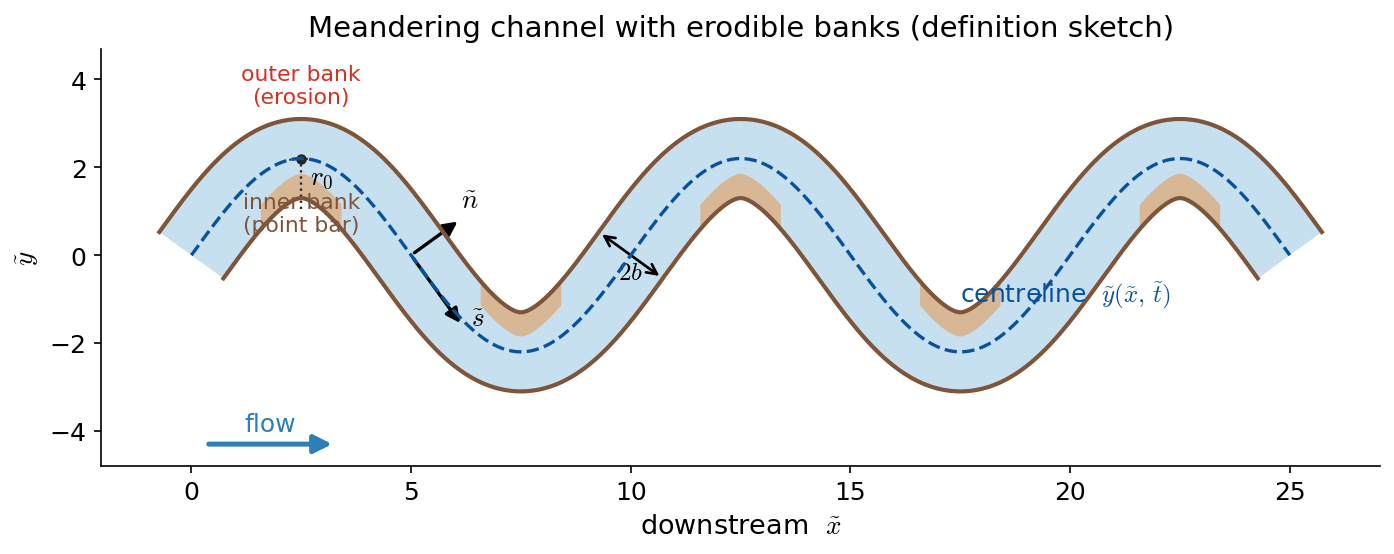
\includegraphics[width=\linewidth]{fig01_planform_definition.png}
    \end{column}
  \end{columns}
  \vfill
  \footnotesize\textcolor{gray}{The paper derives \emph{both} the wavelength and the migration from first principles.}
\end{frame}

\begin{frame}{Two competing ideas: \emph{bar} vs \emph{bend}}
  \begin{columns}[T]
    \begin{column}{0.5\textwidth}
      \textbf{Earlier ``bar'' theories}
      \begin{itemize}
        \item Straight channel, \hl{cBank}{rigid banks}.
        \item Alternate bars form on the bed; flow winds \emph{around} them.
        \item Bank deformation is \emph{not allowed} --- so a true meander cannot develop.
      \end{itemize}
    \end{column}
    \begin{column}{0.5\textwidth}
      \textbf{This paper's ``bend'' theory}
      \begin{itemize}
        \item \hl{cGrowth}{Erodible banks}: the bend itself is unstable.
        \item Curvature $\to$ secondary flow $\to$ selective bank erosion $\to$ growth \emph{and} migration.
        \item Applies to alluvial, incised (bedrock/cave), and glacial meanders alike.
      \end{itemize}
    \end{column}
  \end{columns}
  \vfill
  \centering
  \colorbox{cChannel!10}{\parbox{0.9\linewidth}{\centering
  \textbf{Goal:} a \hl{cChannel}{linear stability analysis} of a sinuous, erodible-bank channel ---
  find the growth rate $\alpha_0(k)$ and migration speed $c_0(k)$ of a small meander perturbation.}}
\end{frame}

\begin{frame}{Roadmap}
  \begin{enumerate}
    \item \textbf{Setup}: geometry, assumptions, the depth-averaged equations.
    \item \textbf{Closures}: secondary flow (the parameter $A$) and a bank-erosion law.
    \item \textbf{The bend equation}: one linear PDE for the centreline $y(x,t)$.
    \item \textbf{Dispersion relation}: growth rate, migration speed, the selected wavelength.
    \item \hl{cEros}{The mechanism}: the curvature\,--\,velocity \emph{phase lag}.
    \item \textbf{Results}: wavelength selection, downstream migration, comparison with data.
  \end{enumerate}
\end{frame}

% ============================================================ 2. SETUP
\section{Setup}

\begin{frame}{Geometry and assumptions}
  \begin{columns}[T]
    \begin{column}{0.5\textwidth}
      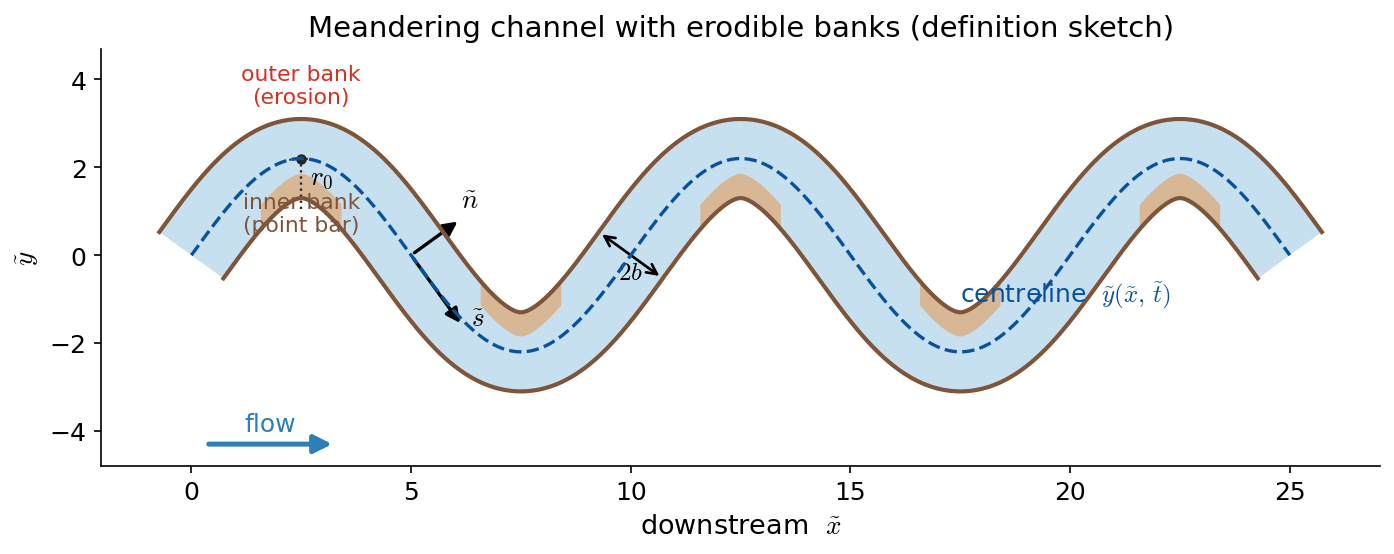
\includegraphics[width=\linewidth]{fig01_planform_definition.png}\\[0.4em]
      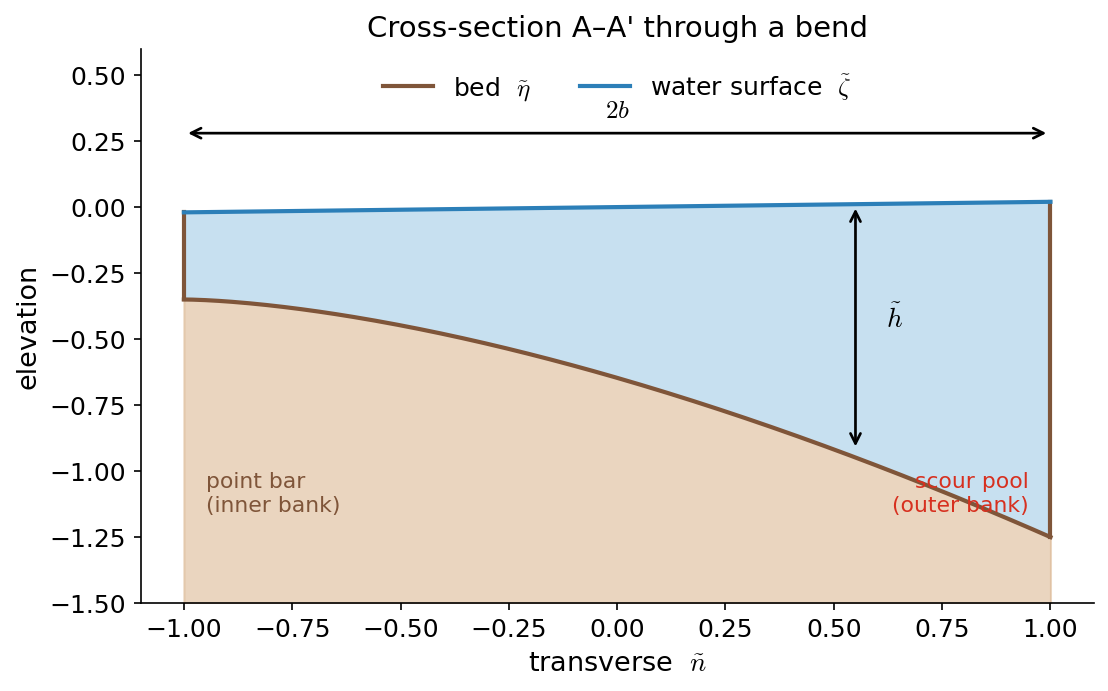
\includegraphics[width=\linewidth]{fig02_cross_section.png}
    \end{column}
    \begin{column}{0.5\textwidth}
      Intrinsic coordinates: $\tilde s$ downstream, $\tilde n$ transverse; centreline
      $\tilde y(\tilde x,\tilde t)$ with curvature $\widetilde{\mathcal C}$.
      \begin{block}{Three assumptions}
        \begin{enumerate}
          \item Constant width $2b$ (erosion $\approx$ deposition).
          \item Gentle bends: $\nu = b/r_0 \ll 1$ (expand to $O(\nu^2)$).
          \item Quasi-steady flow.
        \end{enumerate}
      \end{block}
      Small-amplitude (\emph{linear}) limit: $\delta_0 = k\varepsilon \ll 1$, with
      $\varepsilon = y_0/H_0$, $k = 2\pi H_0/\lambda$.
    \end{column}
  \end{columns}
\end{frame}

\begin{frame}{Governing equations --- depth-averaged St Venant}
  Momentum ($\tilde s,\tilde n$) and continuity for a sinuous channel:
  \begin{align}
    \tilde u\,\partial_{\tilde s}\tilde u + \tilde v\,\partial_{\tilde n}\tilde u
      + \widetilde{\mathcal C}\,\tilde u\tilde v
      &= -g\,\partial_{\tilde s}\tilde\zeta - \tilde\tau_s/(\rho\tilde h), \tag{1a}\\
    \tilde u\,\partial_{\tilde s}\tilde v + \tilde v\,\partial_{\tilde n}\tilde v
      - \widetilde{\mathcal C}\,\tilde u^2
      &= -g\,\partial_{\tilde n}\tilde\zeta - \tilde\tau_n/(\rho\tilde h), \tag{1b}\\
    \widetilde{\mathcal C}\tilde v\tilde h + \partial_{\tilde n}(\tilde v\tilde h)
      + \partial_{\tilde s}(\tilde u\tilde h) &= 0. \tag{1c}
  \end{align}
  Bed stress via a (constant) friction coefficient $C_f$:
  \[
    \tilde\tau_s = \rho C_f\,\widetilde{\mathcal W}\,\tilde u,\qquad
    \tilde\tau_n = \rho C_f\,\widetilde{\mathcal W}\,\tilde v,\qquad
    \widetilde{\mathcal W}=(\tilde u^2+\tilde v^2)^{1/2}.
  \]
  \begin{block}{Zeroth order = uniform flow}
    \[ C_f U^2 = gHI, \qquad UH = q_w \quad(\text{friction balances gravity}).\]
  \end{block}
\end{frame}

% ============================================================ 3. CLOSURES
\section{Closures}

\begin{frame}{Closure 1 --- secondary flow and the parameter $A$}
  \begin{columns}[T]
    \begin{column}{0.5\textwidth}
      The 2-D St Venant system cannot itself capture the \hl{cChannel}{helical
      circulation} in a bend. A 3-D closure (Engelund 1974; \dots) gives, to $O(\nu)$:
      \[ \boxed{\;\dfrac{\eta'}{H} = -A\,\mathcal C'\,\tilde n\;} \tag{6}\]
      \begin{itemize}
        \item Transverse bed slope (and shifted velocity core) $\propto$ curvature.
        \item $A=O(1)$; field data (45 bends): \hl{cGrowth}{$A\simeq 2.89$} for alluvial rivers.
        \item $A=0$ for a laterally flat / incised bed.
      \end{itemize}
    \end{column}
    \begin{column}{0.5\textwidth}
      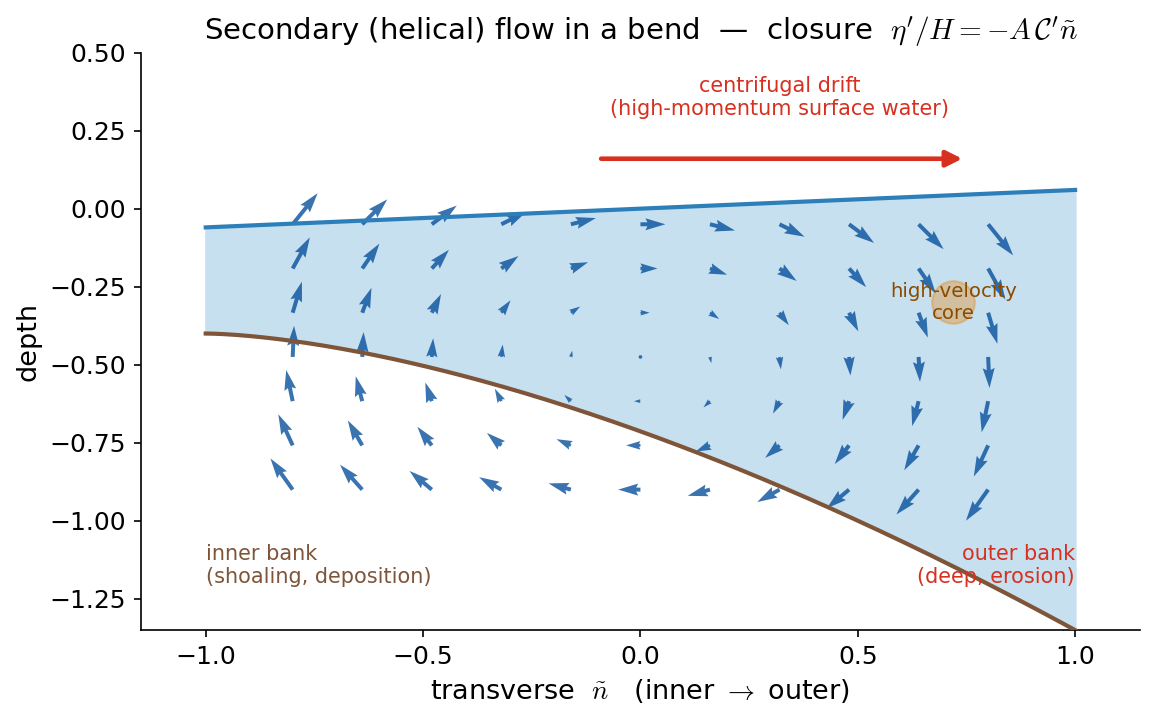
\includegraphics[width=\linewidth]{fig03_secondary_flow.png}
    \end{column}
  \end{columns}
\end{frame}

\begin{frame}{Near-bank velocity --- where the lag is born}
  Substituting the closures into the transverse balance yields a \hl{cVeloc}{forced,
  first-order} equation for the near-bank velocity $u_b=(u')_{\tilde n=b}$
  (linear limit $\chi=\gamma=1$ of Eq.~10):
  \[
    \boxed{\;\frac{\partial u_b}{\partial s} + 2C_f\,u_b
      = b^*\!\left[\,-\,\frac{\partial \mathcal C}{\partial s}
      + C_f\,(A+F^2)\,\mathcal C\,\right]\;}
    \qquad F=\frac{U_0}{\sqrt{gH_0}}.
  \]
  \begin{itemize}
    \item The forcing mixes curvature $\mathcal C$ \emph{and} its along-stream gradient
      $\partial_s\mathcal C$.
    \item A first-order operator with friction damping $2C_f$ $\Rightarrow$ the response
      $u_b$ is \hl{cEros}{phase-shifted} relative to $\mathcal C$: it peaks
      \emph{downstream} of the bend apex.
    \item That shift is the engine of everything that follows.
  \end{itemize}
\end{frame}

\begin{frame}{Closure 2 --- the bank-erosion law}
  \begin{columns}[T]
    \begin{column}{0.52\textwidth}
      Bank migrates at a rate set by the \emph{excess} near-bank velocity:
      \begin{align}
        \gamma\,\partial_{\tilde t}\tilde y &= \tilde\zeta, \qquad \gamma=\cos\theta \tag{11}\\
        \tilde\zeta &= \tilde\zeta(U) + \underbrace{E(U)}_{>0}\,u_b(\tilde s,b) \tag{12}
      \end{align}
      \begin{itemize}
        \item Faster-than-average near-bank flow $\Rightarrow$ erosion; slower $\Rightarrow$ deposition opposite.
        \item Constant width $\Rightarrow$ the whole \emph{centreline} shifts.
        \item The erodibility slope $e=\frac1E\frac{dE}{d\chi}$ matters only at nonlinear order (Part 2).
      \end{itemize}
    \end{column}
    \begin{column}{0.48\textwidth}
      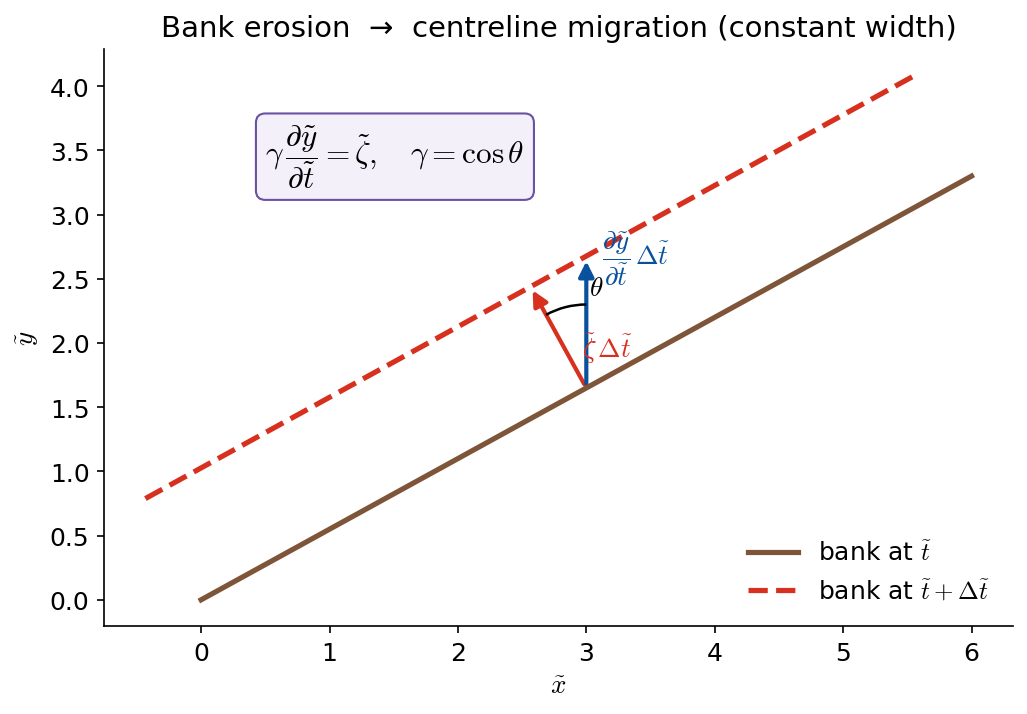
\includegraphics[width=\linewidth]{fig04_bank_erosion.png}
    \end{column}
  \end{columns}
\end{frame}

% ============================================================ 4. BEND EQUATION
\section{The bend equation}

\begin{frame}{Assembling the linearized bend equation}
  Combining the momentum balance, secondary-flow closure and bank-erosion law, and
  transforming to Cartesian coordinates ($\partial_s=\gamma\partial_x$,
  $\mathcal C=-\gamma^3 y_{xx}$), the small-amplitude limit collapses to a single PDE
  for the centreline $y(x,t)$:
  \[
    \boxed{\;\frac{\partial^2 y}{\partial x\,\partial t}
      + 2C_f\,\frac{\partial y}{\partial t}
      = \frac{\partial^3 y}{\partial x^3}
      - C_f\,(A+F^2)\,\frac{\partial^2 y}{\partial x^2}\;} \tag{16}
  \]
  \begin{itemize}
    \item $y_{xt}, y_t$: rate of change of curvature and lateral migration.
    \item $y_{xxx}$: dispersive term from the curvature-gradient forcing.
    \item $-C_f(A+F^2)y_{xx}$: the secondary-flow + Froude driving of growth.
  \end{itemize}
\end{frame}

% ============================================================ 5. DISPERSION
\section{Dispersion relation}

\begin{frame}{Normal modes $\Rightarrow$ the dispersion relation}
  Seek a travelling, growing bend (their Eq.~17):
  \[
    y = \varepsilon\,e^{\alpha_0 t}\cos(kx-\omega_0 t),\qquad
    c_0=\omega_0/k\ \text{(migration speed)}.
  \]
  Substituting into (16) and splitting real/imaginary parts gives
  \begin{align}
    \omega_0 &= \frac{C_f\,k^3\,(2+A+F^2)}{k^2+4C_f^2}, \tag{18a}\\[0.3em]
    \alpha_0 &= \frac{2C_f^2(A+F^2)\,k^2 - k^4}{k^2+4C_f^2}. \tag{18b}
  \end{align}
  \begin{block}{Two immediate readings}
    \small
    Instability ($\alpha_0>0$): \ $k<k_c=\sqrt{2}\,C_f\sqrt{A+F^2}$ \hfill (Eq.~19)\\
    Fastest growth: \ $k_{OM}=\beta C_f$, \ $\beta^2 = 4\sqrt{1+\tfrac12(A+F^2)}-4$ \hfill (Eqs.~20--21)
  \end{block}
\end{frame}

% ============================================================ 6. MECHANISM
\section{The mechanism}

\begin{frame}{The heart of it: the curvature\,--\,velocity phase lag}
  \centering
  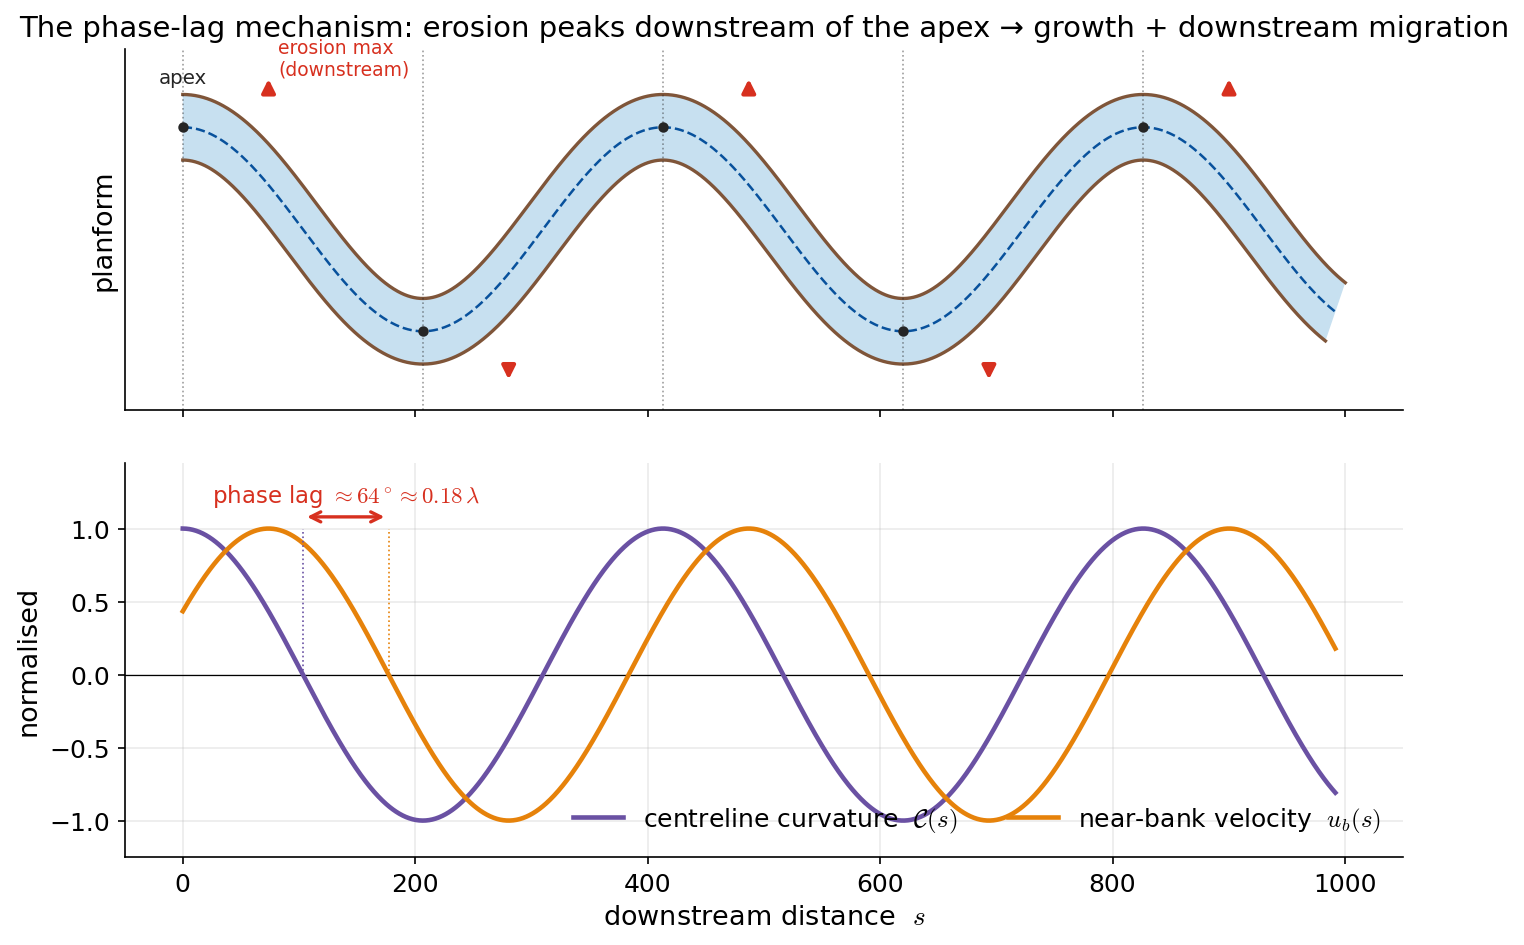
\includegraphics[height=0.66\textheight]{fig05_phase_lag.png}
  \\[0.1em]
  \scriptsize
  Curvature peaks at the apex; near-bank velocity (and erosion) peaks
  \hl{cEros}{$\approx 64^\circ \approx 0.18\lambda$ downstream}
  $\Rightarrow$ the outer bank just past each apex erodes fastest
  $\Rightarrow$ \textbf{growth + downstream migration}.
\end{frame}

\begin{frame}{The mechanism, in motion}
  \begin{columns}[T]
    \begin{column}{0.62\textwidth}
      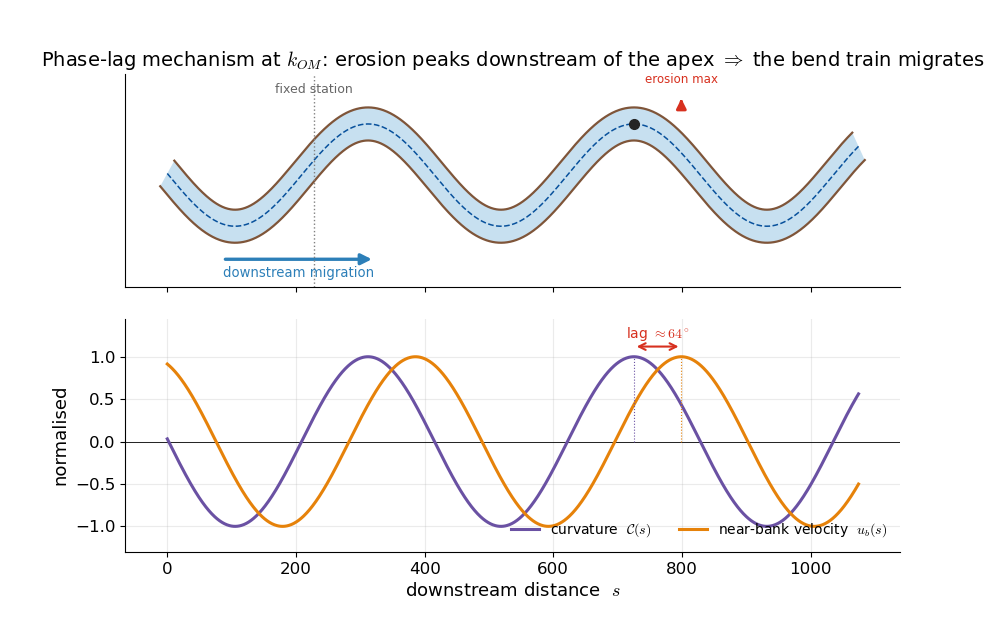
\includegraphics[width=\linewidth]{phase_lag_preview.png}
    \end{column}
    \begin{column}{0.38\textwidth}
      \small
      A travelling bend at $k_{OM}$:
      \begin{itemize}
        \item curvature $\mathcal C(s)$ and near-bank velocity $u_b(s)$ travel together,
        \item separated by the fixed $\sim\!64^\circ$ lag,
        \item so the erosion maximum always rides the downstream flank.
      \end{itemize}
      \playbox{figures/phase\_lag.mp4}
    \end{column}
  \end{columns}
\end{frame}

% ============================================================ 7. RESULTS
\section{Results}

\begin{frame}{Growth rate: a band is unstable, one wavelength wins}
  \begin{columns}[T]
    \begin{column}{0.62\textwidth}
      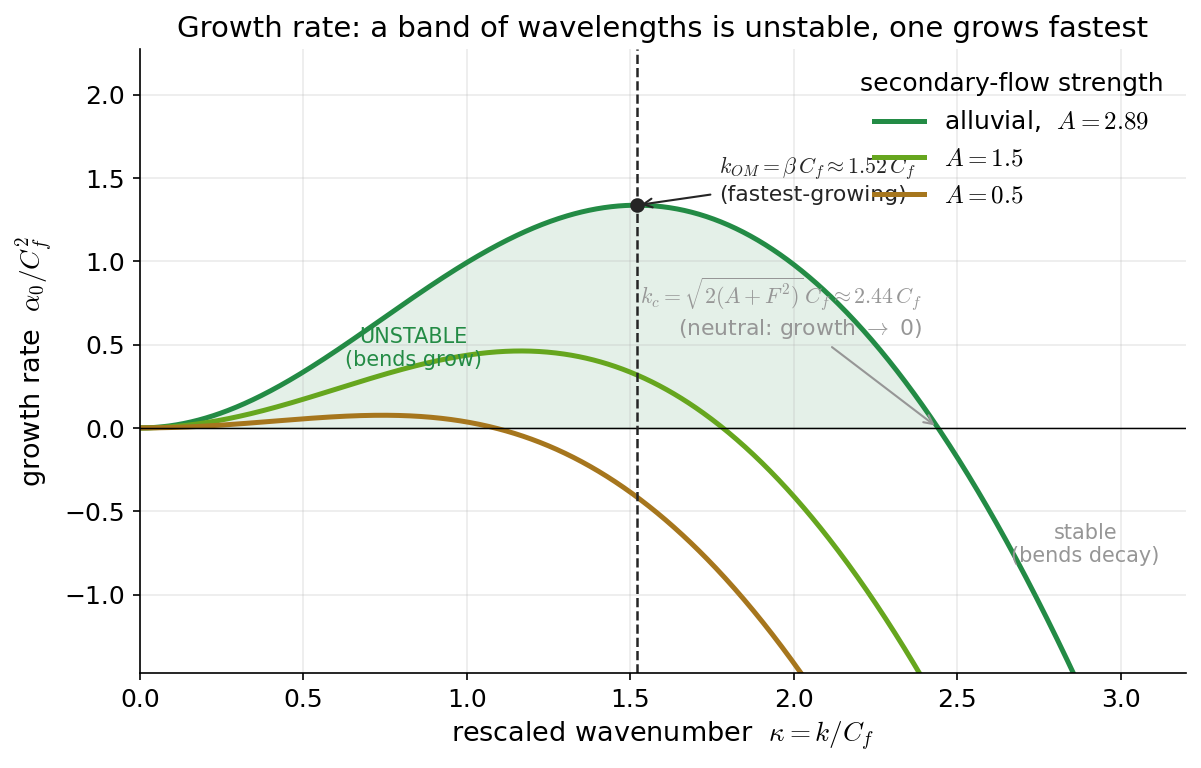
\includegraphics[width=\linewidth]{fig06_growth_rate.png}
    \end{column}
    \begin{column}{0.38\textwidth}
      \small
      In rescaled $\kappa=k/C_f$ the curves are \hl{cChannel}{$C_f$-independent}:
      \[\frac{\alpha_0}{C_f^2}=\frac{2(A{+}F^2)\kappa^2-\kappa^4}{\kappa^2+4}.\]
      \begin{itemize}
        \item Long waves ($\kappa\!\to\!0$): too little forcing.
        \item Short waves ($\kappa>\kappa_c$): friction wins.
        \item Peak at \hl{cEros}{$\kappa_{OM}=\beta$}.
      \end{itemize}
    \end{column}
  \end{columns}
\end{frame}

\begin{frame}{Bends always migrate downstream}
  \begin{columns}[T]
    \begin{column}{0.62\textwidth}
      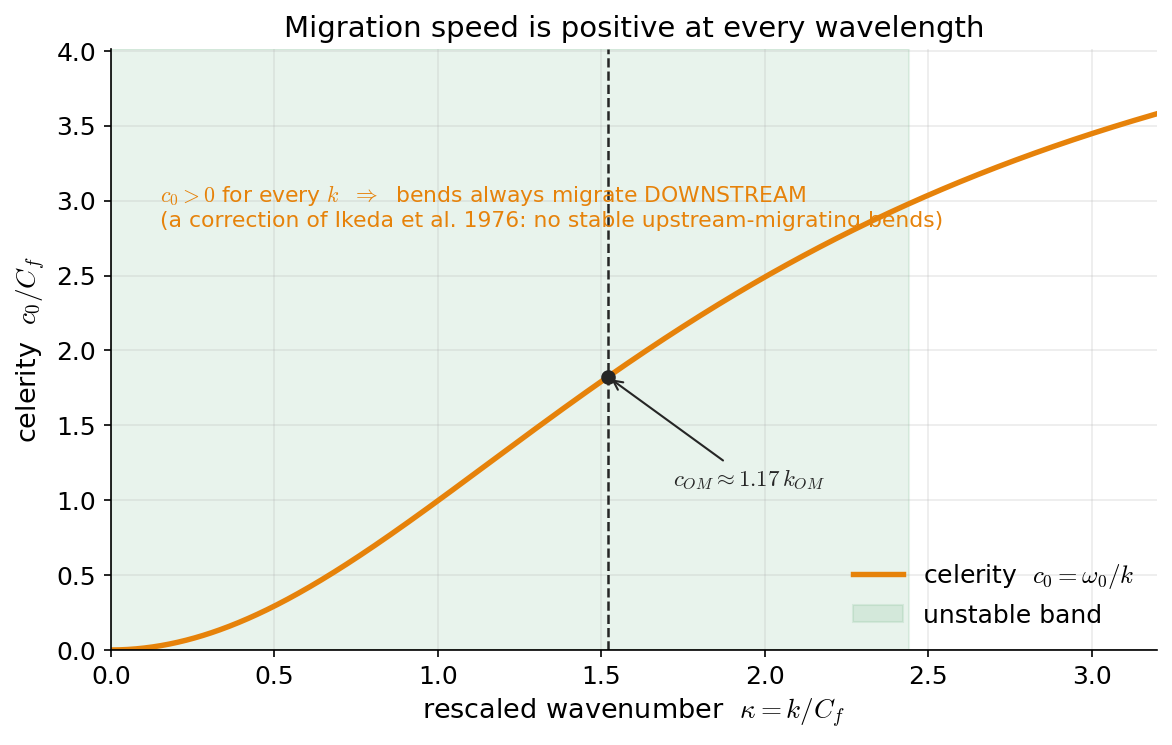
\includegraphics[width=\linewidth]{fig07_celerity.png}
    \end{column}
    \begin{column}{0.38\textwidth}
      \small
      Since $\omega_0>0$ for every $k$, the celerity
      \[ c_0=\frac{C_f\,k^2(2+A+F^2)}{k^2+4C_f^2}>0 \]
      is \hl{cVeloc}{always positive}.
      \begin{itemize}
        \item Bends march \emph{downstream} regardless of Froude number.
        \item Corrects the earlier heuristic (Ikeda et al.\ 1976) that stable bends migrate upstream.
      \end{itemize}
    \end{column}
  \end{columns}
\end{frame}

\begin{frame}{Wavelength selection --- with no fitted constant}
  \centering
  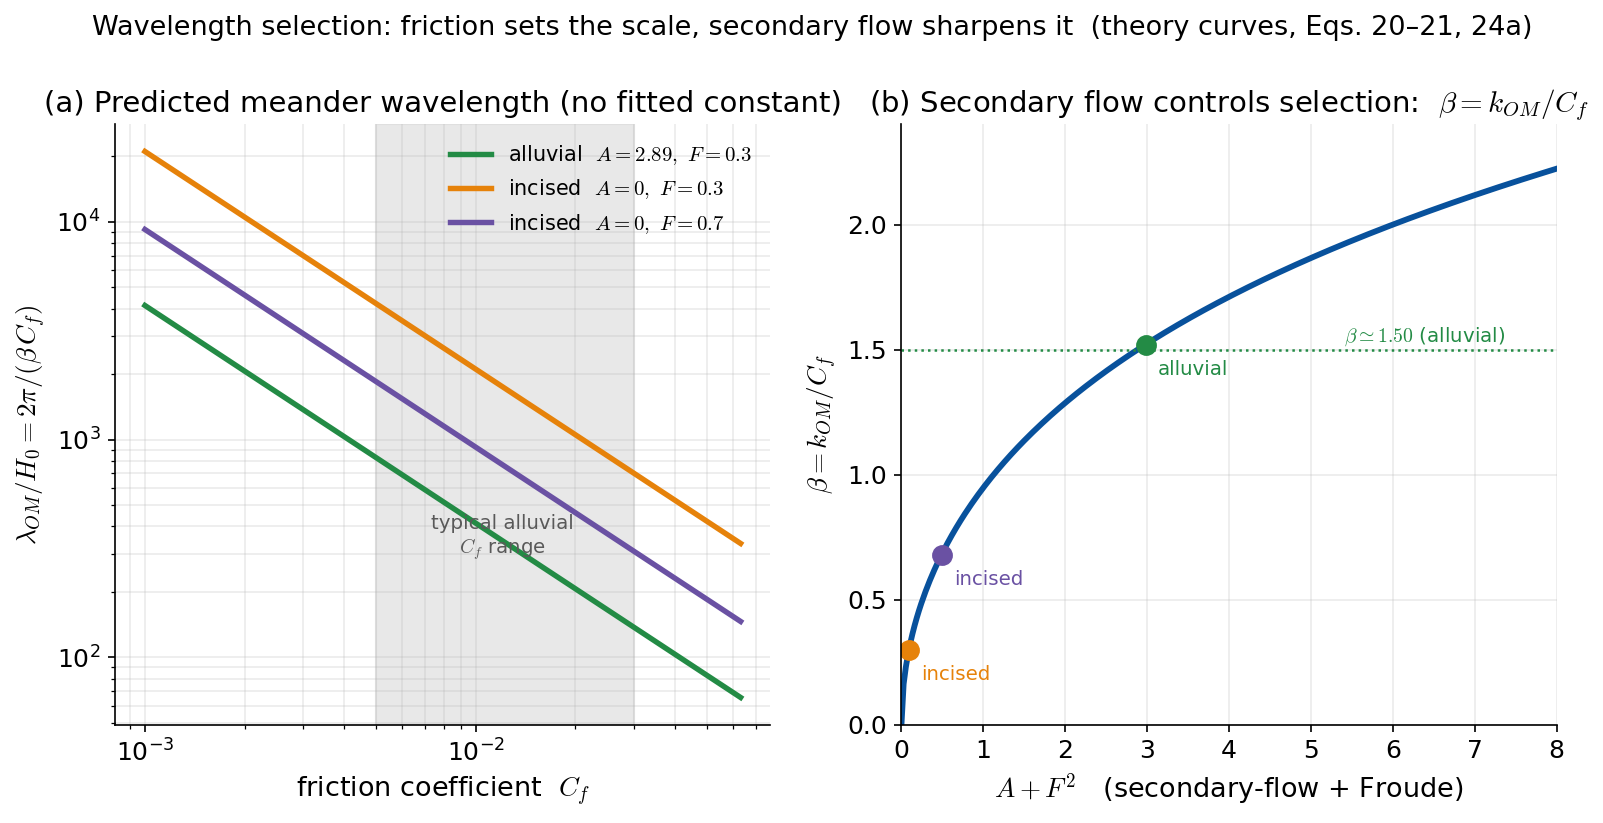
\includegraphics[width=0.95\textwidth]{fig09_wavelength_scaling.png}\\[0.3em]
  \footnotesize
  Alluvial ($A\simeq2.89,\ F^2\!\ll\!A$): $\;k_{OM}=1.50\,C_f$,
  $\ \alpha_{OM}=0.564\,k_{OM}^2,\ \omega_{OM}=1.17\,k_{OM}^2$ (Eqs.~24).\quad
  Incised ($A=0$): $\;k_{OM}\simeq C_f F$ (Eq.~28) $\Rightarrow$ \emph{longer} wavelengths.
\end{frame}

\begin{frame}{How secondary flow reshapes the selection}
  \begin{columns}[T]
    \begin{column}{0.62\textwidth}
      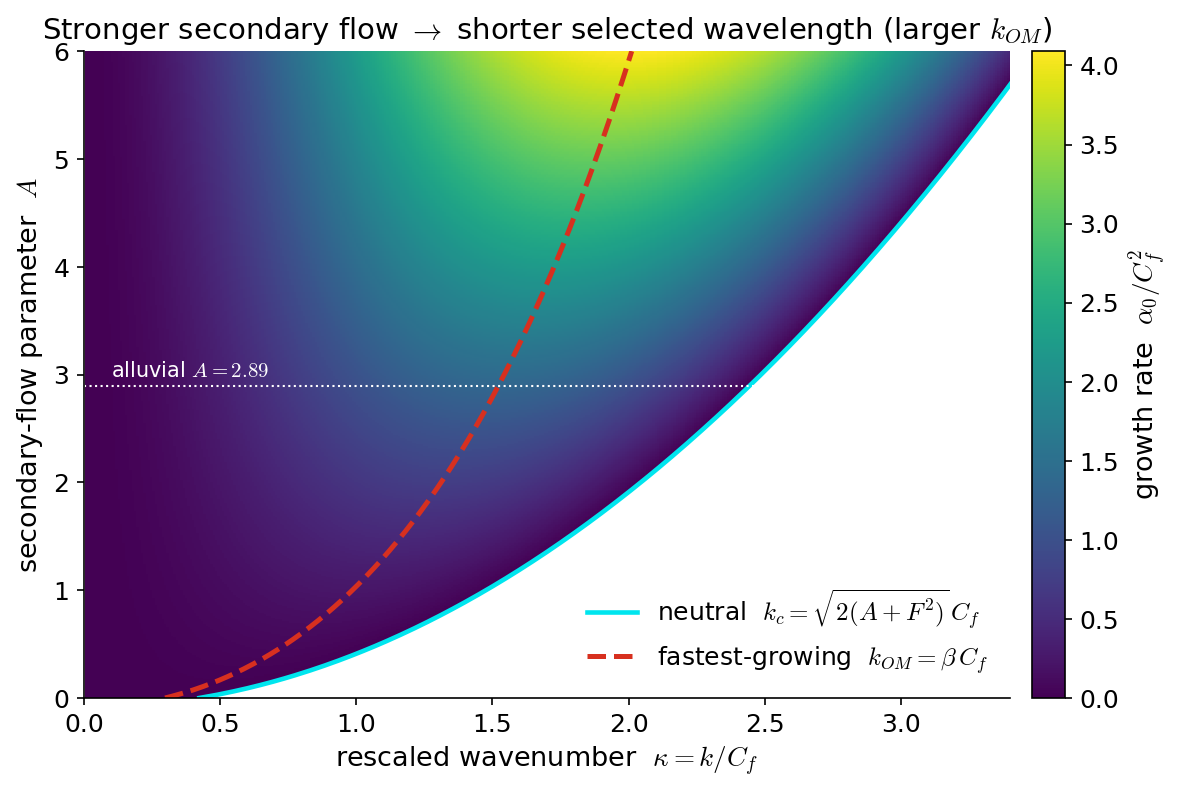
\includegraphics[width=\linewidth]{fig10_sensitivity.png}
    \end{column}
    \begin{column}{0.38\textwidth}
      \small
      Growth rate over $(\kappa, A)$ at fixed $F$:
      \begin{itemize}
        \item stronger secondary flow (larger $A$) $\Rightarrow$ \hl{cEros}{larger $k_{OM}$}
          $\Rightarrow$ \emph{shorter} selected wavelength;
        \item the unstable band widens with $A$;
        \item alluvial rivers sit at $A\approx2.89$.
      \end{itemize}
    \end{column}
  \end{columns}
\end{frame}

\begin{frame}{Secondary flow, animated}
  \begin{columns}[T]
    \begin{column}{0.62\textwidth}
      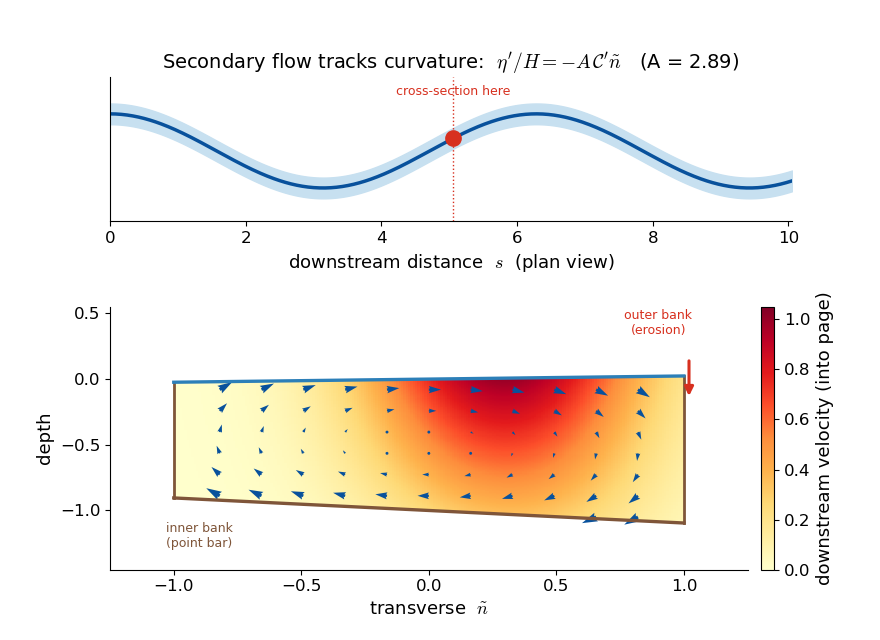
\includegraphics[width=\linewidth]{secondary_flow_preview.png}
    \end{column}
    \begin{column}{0.38\textwidth}
      \small
      Sweeping along the meander, the helical cell, super-elevation, tilted bed and
      outer-bank velocity core all track the local curvature --- and \hl{cEros}{reverse}
      through each inflection.
      \playbox{figures/secondary\_flow.mp4}
    \end{column}
  \end{columns}
\end{frame}

\begin{frame}{From a jumble to a regular train}
  \begin{columns}[T]
    \begin{column}{0.62\textwidth}
      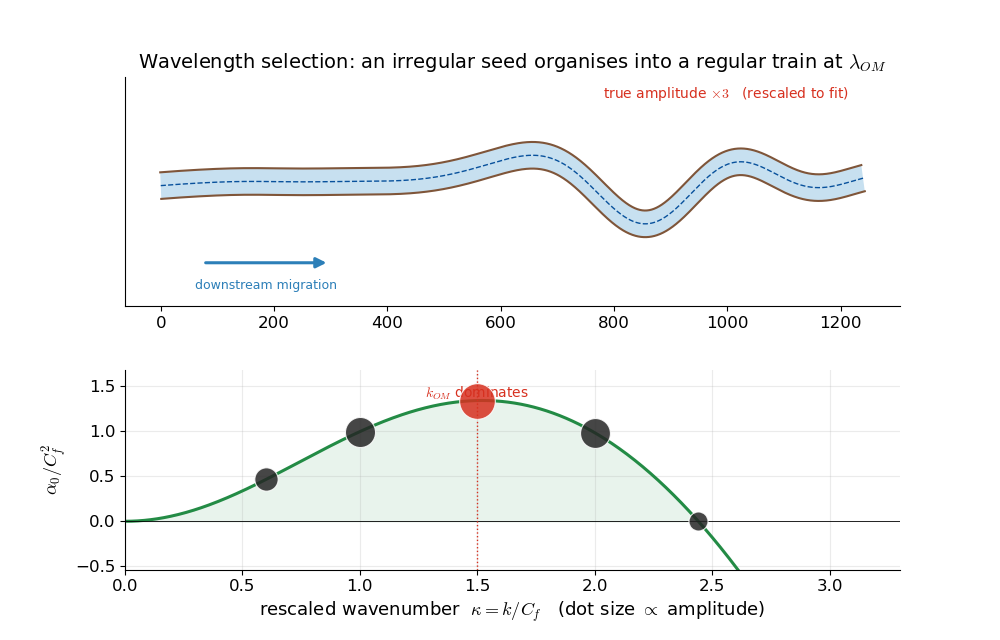
\includegraphics[width=\linewidth]{meander_evolution_preview.png}
    \end{column}
    \begin{column}{0.38\textwidth}
      \small
      Seed the channel with many wavenumbers; each evolves by its own
      $e^{\alpha_0(k)t}\cos(kx-\omega_0 t)$.
      \begin{itemize}
        \item Sub-cutoff modes grow, the rest decay.
        \item The $k_{OM}$ mode overtakes $\Rightarrow$ a \hl{cGrowth}{regular meander train}.
      \end{itemize}
      \playbox{figures/meander\_evolution.mp4}
    \end{column}
  \end{columns}
\end{frame}

\begin{frame}{Comparison with data (theory curves)}
  \begin{itemize}
    \item The paper tests $k_{OM}=1.50\,C_f$ against \textbf{158 laboratory + 73 natural}
      alluvial reaches (their Figs.~4--5): rough agreement over \emph{five decades} of
      wavelength.
    \item Crucially, bend theory carries \hl{cGrowth}{no adjustable constant}, unlike the
      competing bar-theory relation $k_{OM}=aC_f^{1/4}l^{1/4}$ (with fitted $a\simeq0.707$).
    \item Incised cases ($A=0$): rill meanders follow bend theory (Eq.~26a); supraglacial
      meanders look more like bar instability. Cave-stream planforms (Gardner's Gut) show
      the predicted \emph{downstream} migration.
  \end{itemize}
  \vfill
  \centering\footnotesize\itshape
  Here we plot the exact prediction curves rather than reproduce the scatter ---
  the theory has a definite scaling to compare against.
\end{frame}

% ============================================================ 8. WRAP
\section{Wrap-up}

\begin{frame}{Limitations and Part 2}
  \begin{itemize}
    \item Linear theory holds only while $\delta_0=k\varepsilon\ll1$ --- the \emph{early}
      growth of small bends.
    \item As bends fatten, geometric ($\delta_0^3$) and dynamic nonlinearities re-enter:
      amplitude saturation, skewing, and eventually \hl{cEros}{neck cutoff}.
    \item \textbf{Part 2} (Parker, Sawai \& Ikeda 1982) carries the expansion to
      finite amplitude to capture these.
  \end{itemize}
\end{frame}

\begin{frame}{Summary}
  \begin{enumerate}
    \item A sinuous, erodible-bank channel is \hl{cChannel}{linearly unstable}: straight
      channels spontaneously meander.
    \item The mechanism is a \hl{cEros}{phase lag} --- near-bank velocity/erosion peaks
      $\sim0.18\lambda$ downstream of each apex.
    \item This yields a clean \hl{cGrowth}{dispersion relation}: a preferred wavelength
      $k_{OM}=\beta C_f$ and downstream migration $c_0>0$ for all $k$.
    \item For alluvial rivers $\beta\simeq1.50$; the prediction matches data over five
      decades \emph{with no fitted constant}.
    \item Secondary flow (parameter $A$) both drives growth and sets the wavelength.
  \end{enumerate}
  \vfill
  \centering
  \colorbox{cChannel!10}{\parbox{0.92\linewidth}{\centering
  \textbf{One idea to remember:} a small lag between where a river bends and where it flows
  fastest is enough to make meanders \emph{grow} and \emph{march downstream}.}}
\end{frame}

\begin{frame}{Key references}
  \footnotesize
  \begin{itemize}
    \item Ikeda, Parker \& Sawai (1981) \emph{Bend theory of river meanders. Part 1.}
      J.\ Fluid Mech.\ \textbf{112}, 363--377. \hfill(this talk)
    \item Parker, Sawai \& Ikeda (1982) \emph{\dots Part 2. Nonlinear deformation.}
      J.\ Fluid Mech.
    \item Engelund (1974) \emph{Flow and bed topography in channel bends.} J.\ Hydraul.\ Div.\ ASCE \textbf{100}.
    \item Ikeda, Hino \& Kikkawa (1976); Kikkawa, Ikeda \& Kitagawa (1976) --- secondary-flow closures.
    \item Zimmerman \& Kennedy (1978) \emph{Transverse bed slopes in curved alluvial streams.}
    \item Hooke (1975); Leopold, Wolman \& Miller (1964) --- field/lab data.
  \end{itemize}
  \vfill
  \centering\scriptsize\textcolor{gray}{Figures \& animations generated from the verified
  linear relations in \texttt{ikeda\_lib.py}.}
\end{frame}

\end{document}
